% Part 2: predicting the future.
% Build from this directory: make pt2
\documentclass[aspectratio=169,12pt,t]{beamer}
\usepackage{iliad-slides}
\usepackage{tikz}
\usetikzlibrary{arrows.meta,shapes.geometric,fit}
\graphicspath{{figures/}}
\title{Computational Mechanics}
\subtitle{2. Predicting the future}
\institute{ILIAD Intensive}
\date{Autumn 2026}
\author{Xavier Poncini (Simplex)}

\begin{document}
\iliadtitle

\begin{frame}{Outline}
  \vspace{5mm}
  \begin{enumerate}
    \setlength{\itemsep}{4mm}
    \item Sufficient statistics for prediction
    \item Causal states: minimal predictive summaries
    \item Causal-state dynamics
    \item Next-token prediction in RNNs and Transformers
  \end{enumerate}
\end{frame}

\begin{frame}{Predicting the future from the past}
  Let $(X_t)_{t\geq 1}$ be a discrete-time stochastic process on a finite alphabet $\mathcal{X}$.

  \vspace{2mm}

  For consecutive times $i$ to $j$, we introduce the notation:

  \[
    X_{i:j}=(X_i,X_{i+1},\ldots,X_j),
    \qquad
    x_{i:j}=(x_i,x_{i+1},\ldots,x_j)\in\mathcal{X}^{j-i+1}.
  \]

  Consider predicting the \textbf{future} $X_{m+1:m+n}$
  from \textbf{past} observations $X_{1:m}=x_{1:m}$:

  \[
    \Pr\!\left(X_{m+1:m+n}\mid X_{1:m}=x_{1:m}\right).
  \]

  {\centering
    \setlength{\fboxsep}{3mm}
    \setlength{\fboxrule}{0.5pt}
    \fcolorbox{iliadAccent}{white}{%
      \strut How should we do this \textbf{efficiently}?}
    \par}
\end{frame}

% Define predictive sufficiency uniformly across history lengths.
\begin{frame}{Condensing the past}
  \setlength{\parskip}{0pt}
  \setlength{\abovedisplayskip}{4pt}
  \setlength{\belowdisplayskip}{4pt}

  The \textbf{possible histories} are the words that can occur:
  \[
    \mathcal X_+^*
      =\left\{x\in\mathcal X^*\mid \Pr(X_{1:|x|}=x)>0\right\}.
  \]

  \vspace{3mm}
  A \textbf{statistic} maps allowable sequences to summary values:
  \[
    R:\mathcal X_+^*\to\mathcal R.
  \]

  \vspace{3mm}
  $R$ is \textbf{sufficient for prediction} if histories assigned the same
  summary induce the same future distribution:
  \[
    \begin{gathered}
      R(x)=R(x')\quad\Longrightarrow\\[1mm]
      \Pr\!\left(
        X_{|x|+1:|x|+|y|}=y\mid X_{1:|x|}=x
      \right)
      =\Pr\!\left(
        X_{|x'|+1:|x'|+|y|}=y\mid X_{1:|x'|}=x'
      \right).
    \end{gathered}
  \]
  \vspace{3mm}
  This must hold for every $x,x'\in\mathcal X_+^*$ and every
  $y\in\mathcal X^*$.

  \vfill

  \note{This pairwise formulation avoids introducing a decoder. It directly
  requires any two histories mapped to the same summary value to have equal
  probabilities for every finite continuation, even when the histories have
  different lengths. It is equivalent to requiring a common prediction rule
  independent of history length and connects immediately to the later
  definition of causal states.}
\end{frame}

% Sufficiency can retain distinctions that make no predictive difference.
\begin{frame}{Sufficient statistics}
  \setlength{\parskip}{2pt}
  A sufficient statistic can still retain unnecessary distinctions between pasts.

  \vspace{6mm}
  {\centering% A sufficient but non-minimal summary of predictively equivalent histories.
% Same visual language as causal-state-bottleneck.tex on the following slide.
\begin{tikzpicture}[
  x=1mm,y=1mm,
  every node/.style={font=\small,text=iliadInk,align=center},
  summary/.style={draw=iliadAccent,line width=0.6pt,inner sep=2mm,
    minimum width=27mm},
  flow/.style={-{Stealth[length=2mm]},draw=iliadAccent,line width=0.6pt}
]
  \node (pastA) at (10,10) {Past A};
  \node (pastB) at (10,0) {Past B};
  \node (pastC) at (10,-10) {Past C};
  \node[summary] (summaryOne) at (57,10) {Summary $r_1$};
  \node[summary] (summaryTwo) at (57,-5) {Summary $r_2$};
  \node (future) at (112,2) {Same distribution\\over futures};
  \draw[flow] (pastA.east) -- node[midway,fill=white,inner sep=1pt] {$R$} (summaryOne.west);
  \draw[flow] (pastB.east) -- node[midway,fill=white,inner sep=1pt] {$R$} (summaryTwo.west);
  \draw[flow] (pastC.east) -- node[midway,fill=white,inner sep=1pt] {$R$} (summaryTwo.west);
  \draw[flow] (summaryOne.east) -- (future.west);
  \draw[flow] (summaryTwo.east) -- (future.west);
\end{tikzpicture}
\par}

  \vspace{7mm}

  Two summary values give identical predictions: \textbf{sufficient, but not minimal}.

  \vspace{3mm}
  \source{Shalizi, Lecture I (1998), \S3.2; Shalizi \& Crutchfield (2001), \S V.A--B,
  \href{https://arxiv.org/abs/cond-mat/9907176}{cond-mat/9907176}.}

  \note{In this schematic, histories A, B and C all induce exactly the same future
  distribution. Summary $r_1$ retains A separately, while summary $r_2$ groups B and C.
  Both summary values give the correct future distribution, so this distinction
  does not harm sufficiency. But the two values can be merged without changing
  any prediction: the summary is not minimal. The diagram shows only this part
  of the partition, not all possible histories.}
\end{frame}

\begin{frame}{Minimal sufficient statistics}
  \setlength{\parskip}{2pt}
  \textbf{Merge} summary values with identical distributions over futures.

  \vspace{3mm}
  {\centering% The merged version of the sufficient-statistic example on the preceding slide.
\begin{tikzpicture}[
  x=1mm,y=1mm,
  every node/.style={font=\small,text=iliadInk,align=center},
  flow/.style={-{Stealth[length=2mm]},draw=iliadAccent,line width=0.6pt}
]
  \node (pastA) at (10,10) {Past A};
  \node (pastB) at (10,0) {Past B};
  \node (pastC) at (10,-10) {Past C};
  \node[draw=iliadAccent,line width=0.6pt,inner sep=3mm,
    minimum width=27mm,minimum height=13mm] (summary) at (57,0)
    {Merged\\summary $r$};
  \node (future) at (112,0) {Same distribution\\over futures};
  \draw[flow] (pastA.east) -- node[midway,fill=white,inner sep=1pt] {$R_{\min}$} (summary.west);
  \draw[flow] (pastB.east) -- node[midway,fill=white,inner sep=1pt] {$R_{\min}$} (summary.west);
  \draw[flow] (pastC.east) -- node[midway,fill=white,inner sep=1pt] {$R_{\min}$} (summary.west);
  \draw[flow] (summary.east) -- (future.west);
\end{tikzpicture}
\par}
  \vspace{2mm}

  $r_1$ and $r_2$ merge to $r$ under the new statistic $R_{\min}$: predictions are unchanged.

  \vspace{2mm}
  A \textbf{minimal sufficient statistic} gives the
  \textbf{coarsest grouping of pasts} that remains sufficient.
  No two remaining summary values can be merged without changing predictions.

  \source{Shalizi, Lecture I (1998), \S3.2; Shalizi \& Crutchfield (2001), \S V.A--B,
  \href{https://arxiv.org/abs/cond-mat/9907176}{cond-mat/9907176}.}

  \note{This diagram merges the two summary values from the previous slide.
  The three histories have the same predictive distribution for every future
  length, so the merged summary retains all their predictive information.
  Other histories may require other summary values.

  Merging every pair of summary values with identical predictive distributions
  produces the coarsest sufficient partition (up to null histories). A later
  slide names these equivalence classes causal states. As on that slide, the
  requirement concerns futures of every length, rather than only the next token.
  Source: Shalizi and Crutchfield, arXiv:cond-mat/9907176v2, Corollary 1,
  Lemma 7, and Theorem 2, Remark 3.}
\end{frame}

\begin{frame}{Sufficient statistics as partitions}
  \setlength{\parskip}{0pt}
  Sufficient statistics group input sequences with the same future distribution.

  \vspace{4mm}
  {\centering% A finite schematic of a refinement chain, not an exhaustive ordering.
% The same 36 representative words appear in every panel.
\begingroup
\definecolor{predictiveBlue}{HTML}{A9CDE5}
\definecolor{predictiveGold}{HTML}{F2D58A}
\definecolor{predictivePurple}{HTML}{C9B5D8}
\def\sequenceblob{(-18,0)
  .. controls (-20,8) and (-14,15) .. (-6,14)
  .. controls (2,17) and (15,14) .. (17,8)
  .. controls (21,1) and (18,-9) .. (10,-13)
  .. controls (1,-16) and (-12,-14) .. (-16,-8)
  .. controls (-18,-5) and (-19,-2) .. (-18,0) -- cycle}
\begin{tikzpicture}[
  x=1mm,y=0.75mm,
  every node/.style={font=\small,text=iliadInk,align=center},
  boundary/.style={draw=iliadAccent,line width=1pt},
  flow/.style={-{Stealth[length=2mm]},draw=iliadAccent,line width=0.7pt}
]
  \foreach \offset/\stage in {22/0,72/1,122/2} {
    \begin{scope}[shift={(\offset,0)}]
      \begin{scope}
        \clip \sequenceblob;
        \fill[predictiveBlue] (-22,4.5) rectangle (22,18);
        \fill[predictiveGold] (-22,-4.5) rectangle (22,4.5);
        \fill[predictivePurple] (-22,-18) rectangle (22,-4.5);
        \draw[boundary] (-22,4.5) -- (22,4.5);
        \draw[boundary] (-22,-4.5) -- (22,-4.5);
        \ifnum\stage=0
          \foreach \xx in {-11,-5.5,0,5.5,11} {\draw[boundary] (\xx,-18) -- (\xx,18);}
          \foreach \yy in {-9,0,9} {\draw[boundary] (-22,\yy) -- (22,\yy);}
        \fi
        \ifnum\stage=1
          % Unequal, stepped unions of singleton cells within each colour.
          \draw[boundary] (-11,4.5) -- (-11,9) -- (-5.5,9) -- (-5.5,18);
          \draw[boundary] (5.5,4.5) -- (5.5,9) -- (11,9) -- (11,18);
          \draw[boundary] (-5.5,4.5) -- (-5.5,0) -- (0,0) -- (0,-4.5);
          \draw[boundary] (11,4.5) -- (11,0) -- (5.5,0) -- (5.5,-4.5);
          \draw[boundary] (-5.5,-4.5) -- (-5.5,-9) -- (5.5,-9) -- (5.5,-18);
          \draw[boundary] (-5.5,-9) -- (-22,-9);
        \fi
      \end{scope}
      \draw[boundary,line width=1.2pt] \sequenceblob;
      \foreach \xx in {-13.75,-8.25,-2.75,2.75,8.25,13.75} {
        \foreach \yy in {-6.75,-2.25,2.25,6.75,11.25} {
          \fill[iliadInk] (\xx,\yy) circle (0.48mm);
        }
      }
      \foreach \xx in {-8.25,-2.75,2.75,8.25} {
        \fill[iliadInk] (\xx,-11.25) circle (0.48mm);
      }
      % Keep the bottom corner examples inside the curved outer boundary.
      \fill[iliadInk] (-12.5,-10) circle (0.48mm);
      \fill[iliadInk] (12.5,-10) circle (0.48mm);
      \node[font=\footnotesize] at (20,13) {$\mathcal X^*_+$};
    \end{scope}
  }
  \node[font=\small\bfseries] at (22,22) {Finest};
  \node[font=\small\bfseries] at (72,22) {Intermediate};
  \node[font=\small\bfseries] at (122,22) {Coarsest sufficient};
  \node at (22,-22) {$R=\mathrm{id}$\\One sequence per cell};
  \node at (72,-22) {$R$\\Grouped sequences};
  \node at (122,-22) {$R_{\min}$\\Minimal sufficient};
  \draw[flow] (43,0) -- (51,0);
  \draw[flow] (93,0) -- (101,0);
\end{tikzpicture}
\endgroup
\par}

  \vspace{4mm}
  Minimal sufficient statistics are \textbf{memory efficient}.

  \vspace{2mm}
  {\footnotesize\color{iliadMuted}
  Schematic: dots represent example sequences; matching colours indicate identical predictions.\par}
  \note{A statistic induces the partition into its nonempty fibres
  $R^{-1}(r)$. The identity statistic retains the entire word and induces the
  singleton partition. Every sufficient partition refines the minimal
  sufficient partition, up to histories of probability zero.

  Memory efficiency here refers to retained information: a minimal sufficient
  statistic is a function of any other sufficient statistic, so its entropy
  cannot be larger. This does not guarantee finite memory or a particular
  implementation's storage cost. All predictive information is preserved.

  The blobs represent the same set $\mathcal X^*_+$; the 36 dots are a finite
  illustration, not a claim that this set is finite. In the left panel each
  cell represents one word. The middle panel merges unequal groups of cells
  into stepped regions within each predictive class. The right panel merges all cells of each
  colour. Different colours stand for different full future distributions;
  merging across them would lose sufficiency. Three predictive classes are
  illustrative, not a claim that a minimal statistic always has three values.

  The diagram shows one chain in a partial order: two sufficient partitions
  can be incomparable. For words of varying lengths, the predictions are the
  distributions of continuations after each word. The same summary must have
  a common predictive distribution even across lengths. Equivalently, work
  at a fixed observation length as in the preceding sufficiency equation.
  Source: Shalizi and Crutchfield, arXiv:cond-mat/9907176v2, Lemma 7 and
  Theorem 2, Remark 3.}
\end{frame}

% Finite-history causal-state definition following Upper (1997).
\begin{frame}{Causal states}
  \setlength{\parskip}{0pt}
  \setlength{\abovedisplayskip}{4pt}
  \setlength{\belowdisplayskip}{4pt}
  For each $x\in\mathcal X^*_+$, define the map from histories to classes of
  histories by:
  \[
    \resizebox{0.98\textwidth}{!}{$\displaystyle
      \epsilon(x)\equiv
      \left\{x'\in\mathcal X^*_+\;\middle|\;
        \begin{gathered}
          \text{for every }y\in\mathcal X^*,\\[1mm]
          \Pr\!\left(X_{|x|+1:|x|+|y|}=y\mid X_{1:|x|}=x\right)
          =\Pr\!\left(X_{|x'|+1:|x'|+|y|}=y\mid X_{1:|x'|}=x'\right)
        \end{gathered}
      \right\}.
    $}
  \]

  \vfill
  The values of $\epsilon$ are the (finite-history) \textbf{causal states}.

  \vfill
  \textit{``The causal states record every distinction that makes a difference.''}

  \vfill
  \textbf{Theorem.} $\epsilon$ is a minimal sufficient statistic for prediction.

  \textbf{Proof.} We will prove this result in the exercises.

  \vfill
  \source{Upper, \emph{Theory and Algorithms for Hidden Markov Models and
  Generalized Hidden Markov Models} (1997), \S\S2.4--2.5; Shalizi,
  Lecture I (1998), \S3.1.}
  \note{This direct definition does not name the conditional future
  distribution separately. Instead, equality of every finite continuation
  probability appears inside the definition of $\epsilon$.

  The support restriction introduced earlier avoids conditioning on
  zero-probability histories.
  If the process has full support, $\mathcal X^*_+=\mathcal X^*$. The empty
  word belongs to the domain and yields the start-state distribution. Histories
  of different lengths can share a state because both conditional laws begin
  immediately after the observed word.

  Equality for every finite word y is equality on all finite cylinder events,
  and therefore determines the full continuation law. Sufficiency is immediate
  from the definition. If another sufficient statistic R maps x and x' to the
  same value, their continuation laws must agree, so they belong to the same
  $\epsilon$-class. Thus every sufficient partition refines this one.}
\end{frame}

\begin{frame}
  \setlength{\parskip}{0pt}
  \vfill
  \vspace{4mm}
  Past sequences belong to the same causal state when they induce the
  \textbf{same future distribution}.

  \vspace{4mm}
  {\centering% Different histories with the same predictive distribution form one causal state.
\begingroup
\definecolor{tokenBlue}{HTML}{6E9ECC}
\definecolor{tokenGold}{HTML}{E2B857}
\definecolor{tokenCoral}{HTML}{D97D68}
\definecolor{tokenTeal}{HTML}{5DA7A0}
\definecolor{tokenPurple}{HTML}{9B83B5}
\begin{tikzpicture}[
  x=0.92cm,y=0.92cm,
  every node/.style={font=\small,text=iliadInk,align=center},
  flow/.style={-{Stealth[length=2.2mm]},draw=iliadAccent,line width=0.9pt},
  token/.style={draw=white,line width=0.7pt},
  law/.style={draw=iliadInk,line width=0.65pt}
]
  \node[font=\small\bfseries] at (1.55,5.0) {Past (sequences)};
  \node[font=\small\bfseries] at (6.5,5.0) {Future (distribution)};
  \node[font=\small\bfseries] at (11.9,5.0) {Causal state};

  % Four histories: each is a single colour, with width indicating length.
  \node[anchor=east] at (0,4.00) {$x$};
  \filldraw[law,fill=tokenCoral] (0.15,3.76) rectangle (3.30,4.24);

  \node[anchor=east] at (0,3.00) {$x'$};
  \filldraw[law,fill=tokenTeal] (0.85,2.76) rectangle (3.30,3.24);

  \node[anchor=east] at (0,2.00) {$x''$};
  \filldraw[law,fill=tokenPurple] (0.45,1.76) rectangle (3.30,2.24);

  \node[anchor=east] at (0,1.00) {$x'''$};
  \filldraw[law,fill=tokenGold] (1.15,0.76) rectangle (3.30,1.24);

  \draw[dashed,draw=iliadMuted,line width=0.7pt] (3.58,0.52) -- (3.58,4.48);
  \node[font=\scriptsize,text=iliadMuted,rotate=90] at (3.78,2.50) {now};

  % Identical blocks represent the same full predictive distribution.
  \foreach \yy in {4.00,3.00,2.00,1.00} {
    \draw[flow] (3.92,\yy) -- (4.42,\yy);
    \filldraw[law,fill=tokenBlue] (4.55,\yy-0.24) rectangle (8.35,\yy+0.24);
  }

  % The common future law identifies the histories as members of one class.
  \draw[iliadAccent,line width=0.9pt] (8.65,0.76) -- (8.65,4.24);
  \draw[iliadAccent,line width=0.9pt] (8.45,0.76) -- (8.65,0.76);
  \draw[iliadAccent,line width=0.9pt] (8.45,4.24) -- (8.65,4.24);
  \draw[flow] (8.65,2.50) -- (9.55,2.50);

  \path[fill=iliadAccent!7,draw=iliadAccent,line width=1pt]
    (9.72,2.50)
      .. controls (9.55,3.72) and (10.25,4.48) .. (11.35,4.42)
      .. controls (12.50,4.62) and (13.72,3.90) .. (13.72,2.50)
      .. controls (13.92,1.10) and (12.92,0.18) .. (11.72,0.30)
      .. controls (10.52,0.10) and (9.58,1.08) .. (9.72,2.50) -- cycle;

  % Copies of the histories collected inside the causal-state boundary.
  \filldraw[law,fill=tokenCoral]  (10.42,3.48) rectangle (12.53,3.82);
  \filldraw[law,fill=tokenTeal]   (10.85,2.63) rectangle (12.49,2.97);
  \filldraw[law,fill=tokenPurple] (10.61,1.78) rectangle (12.52,2.12);
  \filldraw[law,fill=tokenGold]   (11.05,0.93) rectangle (12.50,1.27);
  \node[font=\footnotesize\bfseries] at (11.72,-0.18)
    {$\epsilon(x)=\epsilon(x')=\epsilon(x'')=\epsilon(x''')$};
\end{tikzpicture}
\endgroup
\par}

  \vspace{0mm}
  {\centering
    \textbf{Same future law} $\Longleftrightarrow$ \textbf{same causal state.}\par}

  \vfill

  \note{Read the diagram from left to right. The coloured token blocks show
  four distinct finite histories, including histories of different lengths.
  Each history induces the same blue block in the middle, which stands for its
  full predictive distribution. The repeated block means equality of those
  predictive laws, not that the future is deterministic. Because the laws
  agree, the four histories are collected into one equivalence class on the
  right.}
\end{frame}

\begin{frame}
  \setlength{\parskip}{0pt}
  \vfill
  \vspace{2mm}
  \textbf{Example 1: (IID process)}

  \vspace{2mm}
  Emits sequences over $\mathcal X=\{0,1\}$ by sampling each symbol
  independently from the same distribution, with both symbols having positive
  probability.

  \vspace{2mm}
  There is one causal state:
  \[
    \epsilon(x)=\left\{(),\ 0,\ 1,\ 00,\ 01,\ 10,\ 11,\ldots\right\}
    =\mathcal X^*_+=\mathcal X^*,
    \qquad x\in\mathcal X^*.
  \]

  \vfill
  \textbf{Example 2: (Golden Mean process)}

  \vspace{2mm}
  Emits sequences over $\mathcal X=\{0,1\}$ in which consecutive $0$s are
  forbidden and, after $1$, either symbol can occur.
  No earlier symbols affect emission probabilities.

  \vspace{2mm}
  For nonempty histories, there are two causal states:
  \[
    \small
    \begin{aligned}
      \epsilon(0)
        &=\left\{0,\ 10,\ 110,\ 010,\ldots\right\}
          =\left\{x\in\mathcal X^*_+\mid x\text{ ends in }0\right\},\\[1mm]
      \epsilon(1)
        &=\left\{1,\ 01,\ 11,\ 101,\ldots\right\}
          =\left\{x\in\mathcal X^*_+\mid x\text{ ends in }1\right\}.
    \end{aligned}
  \]
  \vfill

  \note{For an IID process, conditioning on any observed history leaves every
  finite future distribution unchanged. Consequently every pair of possible
  histories is predictively equivalent and the causal-state partition has a
  single cell. Requiring both symbols to have positive probability gives full
  support, so $\mathcal X^*_+=\mathcal X^*$. The Bernoulli parameter changes
  the common future distribution but not the causal-state partition.

  The Golden Mean process is the standard first-order family. After a 1, the
  process emits 0 with probability q and 1 with probability 1-q, where
  $0<q<1$. After a 0 it emits 1 with probability one. The value of q changes
  the predictive distributions but not the causal-state partition, so it is
  omitted from the visible slide.

  Any two nonempty histories ending in the same symbol have identical future
  laws because the final symbol fixes all subsequent transition
  probabilities. The two displayed classes are distinct because the next
  symbol can be 0 after a history in epsilon(1), but not after a history in
  epsilon(0). Thus a one-step event already separates their full future laws.

  The visible classification is restricted to nonempty histories. The causal
  state of the empty history depends on the process initialization and is not
  shown.}
\end{frame}

\begin{frame}{Updating causal states}
  \setlength{\parskip}{0pt}
  \vfill
  Now consider updating the causal state as the process emits a new token
  $a\in\mathcal X$:

  \vspace{2mm}
  {\centering
  \begin{tikzpicture}[
    x=1cm,y=1cm,
    every node/.style={text=iliadInk},
    flow/.style={-{Stealth[length=2.2mm]},draw=iliadAccent,line width=0.8pt}
  ]
    \node[font=\bfseries,anchor=west] at (7.2,1.6) {Process};
    \node[font=\bfseries,anchor=west] at (7.2,0) {Predictive state};
    \node (x) at (0,1.6) {$x$};
    \node (xa) at (6,1.6) {$xa$};
    \node (epsx) at (0,0) {$\epsilon(x)$};
    \node (epsxa) at (6,0) {$\epsilon(xa)$};
    \draw[flow] (x) -- node[above] {emit $a$} (xa);
    \draw[flow] (x) -- node[left] {$\epsilon$} (epsx);
    \draw[flow] (xa) -- node[right] {$\epsilon$} (epsxa);
    \draw[flow] (epsx) -- node[below] {$\delta(\,\cdot\,,a)$} (epsxa);
  \end{tikzpicture}\par}

  \vfill
  \textbf{Proposition.} The assignment
  \[
    \delta\!\left(\epsilon(x),a\right):=\epsilon(xa),
    \qquad xa\in\mathcal X^*_+,
  \]
  is well-defined: it depends only on the causal state $\epsilon(x)$ and the
  emitted token $a$.

  \vfill
  \vspace{2mm}
  \textbf{Corollary.} Causal-state dynamics form a
  \textbf{partial deterministic automaton}.

  \source{Upper (1997), \S2.4; Shalizi \& Crutchfield (2001),
  \S IV.C, Lemma~5.}
  \vfill

  \note{This variant introduces the update immediately and states the point
  which must be proved. Well-definedness means that changing the representative
  history x without changing epsilon(x) cannot change the destination after
  the same supported token a is appended. The following slide proves exactly
  this claim. The automaton is partial because delta is required only for
  tokens having positive probability from the current state. The automaton's
  states are $\mathcal S=\epsilon(\mathcal X^*_+)$, its alphabet is
  $\mathcal X$, and its transition function is $\delta$.}
\end{frame}

\begin{frame}{Proof of the proposition}
  \setlength{\parskip}{0pt}
  \vfill
  \textbf{Proof.} We must show that the value assigned by
  $\delta(\,\cdot\,,a)$ is independent of the representative chosen from a
  causal state.\par\vspace{2mm}
  Let $x,x'\in\mathcal X^*_+$ satisfy
  $\epsilon(x)=\epsilon(x')$, and suppose $xa\in\mathcal X^*_+$.
  Predictive equivalence gives
  $\Pr(a\mid x)=\Pr(a\mid x')>0$, so $x'a$ is also possible. For every
  $y\in\mathcal X^*$,
  \[
    \Pr(y\mid xa)
      =\frac{\Pr(ay\mid x)}{\Pr(a\mid x)}
      =\frac{\Pr(ay\mid x')}{\Pr(a\mid x')}
      =\Pr(y\mid x'a).
  \]

  \vfill
  Thus $xa$ and $x'a$ induce the same future distribution, so
  $\epsilon(xa)=\epsilon(x'a)$. Therefore $\delta(\,\cdot\,,a)$ assigns the
  same image regardless of the representative chosen from the causal state.
  \hfill$\square$
  \vfill

  \note{The hypothesis that xa lies in the support makes the denominator
  positive. Equality of one-symbol probabilities then makes x'a possible.
  Equality for every continuation ay proves that the extended histories have
  identical predictive laws, so they lie in the same causal state. This is
  exactly the representative-independence asserted by the proposition.}
\end{frame}

\begin{frame}
  \setlength{\parskip}{0pt}
  \vfill
  \vspace{4mm}
  \textbf{Example 1: (IID process)}

  \vspace{2mm}
  Emits sequences over $\mathcal X=\{0,1\}$ by sampling each symbol
  independently from the same distribution, with both symbols having positive
  probability.

  \vspace{0mm}
  {\centering
  \begin{tikzpicture}[
    every node/.style={text=iliadInk,font=\small},
    state/.style={ellipse,draw=iliadAccent,line width=0.9pt,
      fill=iliadAccent!10,minimum width=18mm,minimum height=7mm},
    flow/.style={-{Stealth[length=2mm]},draw=iliadAccent,line width=0.8pt}
  ]
    \node[state] (iid) at (0,0) {$\epsilon(x)$};
    \draw[flow] (iid.north east)
      .. controls +(0.65,0.50) and +(-0.65,0.50) ..
      node[above] {$0,1$} (iid.north west);
  \end{tikzpicture}\par}

  \vfill
  \textbf{Example 2: (Golden Mean process)}

  \vspace{2mm}
  Emits sequences over $\mathcal X=\{0,1\}$ in which consecutive $0$s are
  forbidden and, after $1$, either symbol can occur.
  No earlier symbols affect emission probabilities.

  \vspace{0mm}
  {\centering
  \begin{tikzpicture}[
    every node/.style={text=iliadInk,font=\small},
    state/.style={ellipse,draw=iliadAccent,line width=0.9pt,
      fill=iliadAccent!10,minimum width=18mm,minimum height=7mm},
    flow/.style={-{Stealth[length=2mm]},draw=iliadAccent,line width=0.8pt}
  ]
    \node[state] (one) at (0,0) {$\epsilon(1)$};
    \node[state] (zero) at (3.2,0) {$\epsilon(0)$};
    \draw[flow] (one.north east)
      .. controls +(0.65,0.40) and +(-0.65,0.40) ..
      node[above] {$0$} (zero.north west);
    \draw[flow] (zero.south west)
      .. controls +(-0.65,-0.40) and +(0.65,-0.40) ..
      node[below] {$1$} (one.south east);
    \draw[flow] (one.north west)
      .. controls +(-0.6,0.50) and +(0.6,0.50) ..
      node[above] {$1$} (one.north east);
  \end{tikzpicture}\par}
  \vfill

  \note{These are the same two processes introduced earlier, now shown through
  their causal-state dynamics. Each arrow label is the emitted symbol. For the
  IID process, both symbols return the unique state to itself. For the Golden
  Mean process, 0 moves epsilon(1) to epsilon(0), while 1 moves either state to
  epsilon(1). There is no 0-transition from epsilon(0), because 00 is forbidden.}
\end{frame}

\begin{frame}{Taking stock}
  \setlength{\parskip}{0pt}
  \vfill
  For predicting the \textbf{entire future}:

  \vspace{3mm}
  \begin{itemize}
    \setlength{\itemsep}{3mm}
    \item Causal states are the \textbf{most efficient summary of the past}.
    \item Given a new observation, the causal state is \textbf{easy to update}.
  \end{itemize}

  \vfill
  {\centering
    \setlength{\fboxsep}{4mm}
    \setlength{\fboxrule}{0.6pt}
    \fcolorbox{iliadAccent}{iliadAccent!6}{%
      \parbox{0.84\textwidth}{\centering
        But modern autoregressive neural networks do not predict the entire
        future directly. They predict \textbf{only the next-token distribution}.}}
    \par}
  \vfill

  \note{Here, ``most efficient'' means minimal sufficient for predicting the full
  continuation law. The deterministic update established above makes this
  summary easy to maintain as observations arrive. The contrast motivates the
  next question: if a model is trained only on next-token probabilities, which
  distinctions between pasts must its internal state retain?}
\end{frame}

\begin{frame}{Recurrent next-token prediction}
  \setlength{\parskip}{0pt}
  \vfill
  Given hidden state $h_{n-1}$ and observation $x_n$, a model with parameters
  $\theta$ recurrently updates its hidden state and produces prediction $y_n$:

  \vspace{-3mm}
  \[
    h_n=f_\theta(h_{n-1},x_n),
    \qquad
    y_n=g_\theta(h_{n-1},x_n).
  \]

  \textbf{Proposition.} Fix the initial hidden state $h_0$. Suppose that, for
  every $n\geq 1$,
  \[
    y_n
      =\Pr\!\left(
        X_{n+1}\mid X_{1:n}=x_{1:n}
      \right),
      \qquad \forall\,x_{1:n}\in\mathcal X_+^*.
  \]
  Then the recurrent state $(h_{n-1},x_n)$ is a sufficient statistic for the
  entire future.

  \vfill
  \vspace{2mm}
  {\centering
    \setlength{\fboxsep}{2.5mm}
    \setlength{\fboxrule}{0.6pt}
    \fcolorbox{iliadAccent}{iliadAccent!6}{%
      \parbox{0.84\textwidth}{\centering
        Exact recurrent \textbf{next-token prediction}\\[1mm]
        $\Longrightarrow$ a sufficient statistic for the \textbf{entire future!}}}
    \par}

  \vspace{2mm}
  \source{Shalizi (2001), Theorem~6; Shalizi \& Shalizi (2004), \S2.}
  \vfill

  \note{The indexing emphasizes the Mealy timing convention. The hidden state
  h_{n-1} summarizes the observations through x_{n-1}. When x_n arrives, the same
  state--input pair produces both the updated hidden state h_n and the
  distribution used to predict X_{n+1}. The dot indicates that y_n is the
  whole probability distribution on the finite alphabet, rather than a single
  probability or an argmax prediction. The proposition applies to the pair
  $(h_{n-1},x_n)$, which is the predictive state in the Mealy convention and
  is itself recurrently updated.}
\end{frame}

\begin{frame}{Why is next-token prediction enough?}
  \setlength{\parskip}{0pt}
  \vfill
  We leave the proof as an exercise and provide the intuition here.

  \vspace{4mm}
  Let $r_n:=(h_{n-1},x_n)$ and
  $y_n:=\Pr(X_{n+1}\mid X_{1:n}=x_{1:n})$. The recurrent update determines
  the entire future distribution via next-token probabilities:
  \begin{center}
    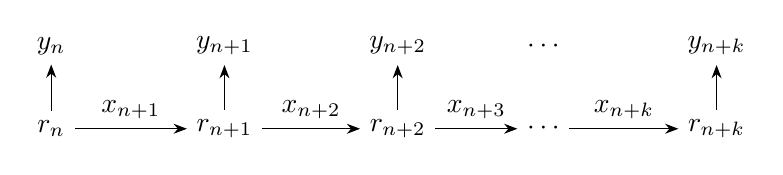
\begin{tikzpicture}[>=Stealth]
      \node (rn) at (0,0) {$r_n$};
      \node (rn1) at (2.2,0) {$r_{n+1}$};
      \node (rn2) at (4.4,0) {$r_{n+2}$};
      \node (dots) at (6.25,0) {$\cdots$};
      \node (rnk) at (8.45,0) {$r_{n+k}$};

      \node (yn) at (0,1.05) {$y_n$};
      \node (yn1) at (2.2,1.05) {$y_{n+1}$};
      \node (yn2) at (4.4,1.05) {$y_{n+2}$};
      \node (ydots) at (6.25,1.05) {$\cdots$};
      \node (ynk) at (8.45,1.05) {$y_{n+k}$};

      \draw[->] (rn) -- (yn);
      \draw[->] (rn1) -- (yn1);
      \draw[->] (rn2) -- (yn2);
      \draw[->] (rnk) -- (ynk);
      \draw[->] (rn) -- node[above] {$x_{n+1}$} (rn1);
      \draw[->] (rn1) -- node[above] {$x_{n+2}$} (rn2);
      \draw[->] (rn2) -- node[above] {$x_{n+3}$} (dots);
      \draw[->] (dots) -- node[above] {$x_{n+k}$} (rnk);
    \end{tikzpicture}
  \end{center}

  \vspace{3mm}
  Information in the past $x_{1:n}$ inducing a future distinction
  must be stored in $r_n$.

  \vfill
  \source{A. Shai (2026), private communication.}

  \note{Fixing a continuation recursively fixes every future recurrent state.
  The state at each step supplies the exact distribution of the following
  token. Consequently the initial recurrent state determines the probability
  assigned to every finite continuation, which is precisely sufficiency for
  the entire future. The formal induction is left as an exercise.}
\end{frame}

\begin{frame}{What about transformers?}
  \setlength{\parskip}{0pt}
  \only<1>{%
    \vfill
    {\centering
      \resizebox{0.45\textwidth}{!}{%
        \begin{tikzpicture}[
  x=1cm,y=1cm,
  every node/.style={text=iliadInk,font=\small},
  token/.style={draw=iliadInk,line width=0.6pt,minimum width=9mm,
    minimum height=7mm,fill=white},
  output/.style={draw=iliadInk,line width=0.6pt,minimum width=9mm,
    minimum height=7mm,fill=white},
  block/.style={draw=iliadAccent,line width=0.8pt,fill=iliadAccent!16,
    minimum width=62mm,minimum height=6mm},
  vflow/.style={-{Stealth[length=1.8mm]},draw=iliadInk,line width=0.6pt},
  hflow/.style={-{Stealth[length=2mm]},draw=iliadAccent,line width=0.8pt}
]
  \foreach \yy in {1.15,2.55,3.95}{
    \node[block] at (3,\yy) {};
    \draw[hflow] (0.35,\yy) -- (5.65,\yy);
  }

  \foreach \xx/\lab/\id in {0.65/$x_1$/one,2.05/$x_2$/two,
      3.95/$x_n$/n,5.35/$x_{n+1}$/new}{
    \node[token] (barein\id) at (\xx,0) {\lab};
    \draw[vflow] (barein\id.north) -- (\xx,0.82);
    \draw[vflow] (\xx,1.48) -- (\xx,2.22);
    \draw[vflow] (\xx,2.88) -- (\xx,3.62);
    \draw[vflow] (\xx,4.28) -- (\xx,4.82);
  }
  \node at (3,0) {$\cdots$};

  \foreach \xx/\lab/\id in {0.65/$y_1$/one,2.05/$y_2$/two,
      3.95/$y_n$/n,5.35/$y_{n+1}$/new}{
    \node[output] (bareout\id) at (\xx,5.17) {\lab};
  }
  \node at (3,5.17) {$\cdots$};
\end{tikzpicture}
}
      \par}
    \vfill
  }

  \only<2>{%
    \vfill
    {\centering
      \resizebox{0.77\textwidth}{!}{%
        \begin{tikzpicture}[
  x=1cm,y=1cm,
  every node/.style={text=iliadInk,font=\scriptsize},
  token/.style={draw=iliadInk,line width=0.55pt,minimum width=7mm,
    minimum height=6mm,fill=white},
  output/.style={draw=iliadInk,line width=0.55pt,minimum width=7mm,
    minimum height=6mm,fill=white},
  block/.style={draw=iliadAccent,line width=0.7pt,fill=iliadAccent!16,
    minimum width=48mm,minimum height=5mm},
  vflow/.style={-{Stealth[length=1.5mm]},draw=iliadInk,line width=0.55pt},
  hflow/.style={-{Stealth[length=1.8mm]},draw=iliadAccent,line width=0.75pt},
  cachefill/.style={fill=purple!5},
  cacheoutline/.style={draw=purple!70!black,line width=0.8pt,fill=none},
  cachelabel/.style={draw=purple!70!black,line width=0.8pt,
    fill=purple!7,rounded corners=0.7mm,inner xsep=2mm,inner ysep=1mm},
  highlight/.style={draw=purple!70!black,line width=0.8pt,inner sep=1.3mm}
]

% Cache before processing the new token.
\begin{scope}
  \path[cachefill] (-0.2,0.75) rectangle (3.55,3.75);
  \foreach \yy in {1.05,2.25,3.45}{
    \node[block] (L\yy) at (2.25,\yy) {};
    \draw[hflow] (0.18,\yy) -- (4.32,\yy);
  }

  \foreach \xx/\lab/\id in {0.45/$x_1$/one,1.55/$x_2$/two,
      3.05/$x_n$/n,4.35/$x_{n+1}$/new}{
    \node[token] (tin\id) at (\xx,0) {\lab};
    \draw[vflow] (tin\id.north) -- (\xx,0.78);
    \draw[vflow] (\xx,1.32) -- (\xx,1.98);
    \draw[vflow] (\xx,2.52) -- (\xx,3.18);
    \draw[vflow] (\xx,3.72) -- (\xx,4.20);
  }
  \node at (2.30,0) {$\cdots$};

  \foreach \xx/\lab/\id in {0.45/$y_1$/one,1.55/$y_2$/two,
      3.05/$y_n$/n,4.35/$y_{n+1}$/new}{
    \node[output] (out\id) at (\xx,4.50) {\lab};
  }
  \node at (2.30,4.50) {$\cdots$};
  \draw[cacheoutline] (-0.2,0.75) rectangle (3.55,3.75);
  \node[cachelabel,text=purple!70!black,font=\small\bfseries] at (1.68,2.84)
    {$h_n=\mathrm{KV}_{1:n}$};
  \foreach \xx/\id in {0.45/one,1.55/two,3.05/n,4.35/new}{
    \draw[vflow] (tin\id.north) -- (\xx,0.78);
    \draw[vflow] (\xx,3.72) -- (\xx,4.20);
  }
  \node[highlight,fit=(tinnew)] {};
\end{scope}

% One cached decoding step.
\draw[-{Stealth[length=2.5mm]},draw=iliadAccent,line width=1pt]
  (5.25,2.45) -- (7.15,2.45);
\node[font=\small] at (6.20,2.86) {$f_\theta,\,g_\theta$};
\node[font=\scriptsize,text=iliadMuted] at (6.20,2.05)
  {one forward pass};

% Expanded cache and the newly produced next-token distribution.
\begin{scope}[shift={(8,0)}]
  \path[cachefill] (-0.2,0.75) rectangle (4.65,3.75);
  \foreach \yy in {1.05,2.25,3.45}{
    \node[block] (R\yy) at (2.25,\yy) {};
    \draw[hflow] (0.18,\yy) -- (4.32,\yy);
  }

  \foreach \xx/\lab/\id in {0.45/$x_1$/one,1.55/$x_2$/two,
      3.05/$x_n$/n,4.35/$x_{n+1}$/new}{
    \node[token] (rtin\id) at (\xx,0) {\lab};
    \draw[vflow] (rtin\id.north) -- (\xx,0.78);
    \draw[vflow] (\xx,1.32) -- (\xx,1.98);
    \draw[vflow] (\xx,2.52) -- (\xx,3.18);
    \draw[vflow] (\xx,3.72) -- (\xx,4.20);
  }
  \node at (2.30,0) {$\cdots$};

  \foreach \xx/\lab/\id in {0.45/$y_1$/one,1.55/$y_2$/two,
      3.05/$y_n$/n,4.35/$y_{n+1}$/new}{
    \node[output] (rout\id) at (\xx,4.50) {\lab};
  }
  \node at (2.30,4.50) {$\cdots$};
  \draw[cacheoutline] (-0.2,0.75) rectangle (4.65,3.75);
  \node[cachelabel,text=purple!70!black,font=\small\bfseries] at (2.25,2.84)
    {$h_{n+1}=\mathrm{KV}_{1:n+1}$};
  \foreach \xx/\id in {0.45/one,1.55/two,3.05/n,4.35/new}{
    \draw[vflow] (rtin\id.north) -- (\xx,0.78);
    \draw[vflow] (\xx,3.72) -- (\xx,4.20);
  }
  \node[highlight,fit=(routnew)] {};
\end{scope}

\end{tikzpicture}
}
      \par}

    \vspace{4mm}
    {\centering
      \setlength{\fboxsep}{2mm}
      \setlength{\fboxrule}{0.6pt}
      \fcolorbox{iliadAccent}{iliadAccent!6}{%
        \parbox{0.82\textwidth}{\centering
          Transformer with \textbf{exact next-token prediction}\\[1mm]
          $\Longrightarrow\quad (h_n,x_{n+1})$ is sufficient for
          \textbf{the entire future!}}}
      \par}

    \source{Dai et al. (2019); Katharopoulos et al. (2020, linear attention);\
    A. Kolchinsky (2026), private communication.}
    \vfill
  }

  \note{The first view recalls the ordinary causal Transformer computation
  without assigning it a recurrent state. The second view identifies the KV
  cache as that state. Read the left panel as the cached state before the new token has been
  incorporated. The full KV cache h_n and the incoming token x_{n+1} determine
  both the expanded cache h_{n+1} and the next-token distribution y_{n+1} in
  one deterministic forward pass. This is exactly the recurrent form introduced
  above. Therefore, if the Transformer is exact on every supported
  history, the pair (h_n,x_{n+1}) is sufficient for the entire future. The
  cache can retain more information than the causal state; the claim is that
  the causal state is recoverable from it. A finite context window can satisfy
  the premise only when the retained context is itself sufficient.
  Transformer-XL supplies the precedent for treating cached activations as
  recurrent memory. Katharopoulos et al. give an explicit recurrent
  formulation for linear-attention Transformers; the ordinary softmax
  Transformer shown here instead has a cache whose size grows with the
  sequence.}
\end{frame}

\begin{frame}{Do neural networks learn causal states?}
  \setlength{\parskip}{0pt}
  \vfill

  Recurrent neural networks and Transformers that achieve exact next-token
  prediction develop \textbf{sufficient statistics} for the entire future!

  \vspace{10mm}
  \textbf{Why might these sufficient statistics also be minimal?}

  \vspace{3mm}
  \textbf{Simplicity bias:} Capacity constraints and regularisation favour
  simpler representations that discard distinctions irrelevant to prediction.

  \vspace{9mm}
  \textbf{How might a neural network encode the structure of a causal state?}

  \vspace{3mm}
  In the following lecture, we will turn to this question.

  \vfill

  \note{The sufficiency statement follows from the preceding results under
  exact next-token prediction. Minimality does not follow automatically:
  a network may preserve distinctions that are irrelevant to prediction.
  Simplicity bias, finite capacity, and regularisation motivate the hypothesis
  that trained networks tend to compress such distinctions. If this compression
  reaches the minimal sufficient statistic, the resulting representation is
  equivalent to the causal-state partition up to an invertible relabelling.}
\end{frame}

\begin{frame}{Summary}
  \setlength{\parskip}{0pt}
  \vfill

  \textbf{For predicting the entire future:}

  \vspace{2mm}
  \begin{itemize}
    \item Causal states are the \textbf{most efficient summary of the past}.
    \item Given a new observation, the causal state is \textbf{easy to update}.
  \end{itemize}

  \vspace{7mm}
  \textbf{For next-token prediction:}

  \vspace{2mm}
  \begin{itemize}
    \item Recurrent neural networks and Transformers that achieve exact
      next-token prediction develop \textbf{sufficient statistics} for the
      entire future.
    \item Simplicity bias suggests that these learned statistics may approach
      \textbf{minimal sufficient statistics}.
  \end{itemize}

  \vfill
\end{frame}


\end{document}
